\documentclass{article}
\usepackage[italian]{babel}
\usepackage[utf8]{inputenc}
\usepackage[T1]{fontenc}
\usepackage{float}
\usepackage{amsmath}
\usepackage{nicefrac}
\usepackage{graphicx}
\usepackage{multicol}
\usepackage{fancyhdr}
\usepackage[export]{adjustbox}
\usepackage{geometry}
\usepackage{caption}
\usepackage{subcaption}
\usepackage{graphicx}


\usepackage{blindtext}
\geometry{
	a4paper,
	total={170mm,257mm},
	left=20mm,
	top=20mm,
}

\begin{document}
\noindent\Huge\textmd{\textbf{Simulazione e ricostruzione di vertice}}
\newline\noindent\large Maria Susini, Elisa Visentin 
\newline\newline\noindent
Scopo del programma è studiare la propagazione delle particelle cariche generate dalla collisione di due fasci di particelle attraverso un apparato sperimentale costituito dalla beam pipe e da due layer di rivelatori. Segue la descrizione della routine di esecuzione del codice e della sua struttura. In conclusione sono riportati i risultati ottenuti.
\newline\noindent\rule{17cm}{0.1pt}
\section{Esecuzione del codice}
Per avviare il programma completo di simulazione e ricostruzione occorre seguire le seguenti istruzioni:
\begin{itemize}
	\item .L compilevertex.C
	\item compilevertex(): comando per compilare le classi e le macro custom necessarie ad eseguire la simulazione, la ricostruzione e la successiva analisi
	\item simulazione(): comando per eseguire la parte di simulazione e salvare i risultati nel tree in "simulazione.root"
	\item ricostruzione(): comando per eseguire la ricostruzione di vertice per ogni evento generato e salvare i risultati del processamento nel file "ricostruzione.root" (contiene anche la funzione \textit{plot} utilizzata per analizzare i risultati)
	\item canvasses(): comando per disegnare gli istogrammi che rappresentano i risultati ottenuti. 
\end{itemize}


\section{Descrizione classi e macro implementate}
In questo paragrafo si descrivono le caratteristiche principali delle classi e delle macro utilizzate per la simulazione e la ricostruzione. Le classi implementate sono \textit{Vertex}, \textit{Track} e \textit{Intpoint}; le macro sono \textit{simulazione}, \textit{ricostruzione} e \textit{canvasses}.

\subsection{Classe Vertex}
La classe \textit{Vertex} viene utilizzata per generare le tre coordinate cartesiane del vertice di interazione, la molteplicità (numero di particelle cariche prodotte a seguito della collisione) e le relative direzioni di propagazione.
\\
I data member di questa classe sono le coordinate cartesiane \textit{fX,fY,fZ} del vertice, la molteplicità ed esso associata \textit{fMulti} e gli angoli polare e azimutale \textit{fTheta} e \textit{fPhi} che indicano la direzione di propagazione della particella carica generata. Fanno parte dei member function private la funzione \textit{Var}, che permette di impostare i valori delle coordinate cartesiante tramite Box-Muller, e le funzioni \textit{Multunif} e \textit{Multfunc} con le quali è possibile fissare la molteplicità associata al vertice. Nel primo caso la molteplicità è estratta da una distribuzione uniforme, nel secondo da una distribuzione assegnata rappresentata da un istogramma.
\\
Per quanto riguarda le member function pubbliche, oltre ai costruttori di default, standard e copia, si hanno delle funzioni \textit{Get} che sono utilizzate per accedere ai data members. Si ha poi la funzione \textit{Initialdir} per inizializzare il valore di \textit{fTheta} e \textit{fPhi}; il primo è assegnato a partire da una distribuzione nota in pseudorapidità e il secondo è estratto uniforme nell'intervallo [0,2$\pi$].

\subsection{Classe Track}
La classe \textit{Track} viene utilizzata per generare la traccia della particella carica noti gli angoli di propagazione iniziali e individuare il suo punto di intersezione con i diversi layer di cui è composto l'apparato sperimentale. 
\\
I data member di questa classe sono i coseni direttori \textit{fC1}, \textit{fC2} e \textit{fC3} della retta e gli angoli \textit{fTheta} e \textit{fPhi} che le funzioni implementate nella classe aggiornano. \\
Per quanto riguarda le member function, si ha una funzione \textit{Parameter} per stimare il valore del parametro \textit{t} della retta. Questa viene poi utilizzata nella funzione \textit{Intersection} al fine di valutare il valore delle coordinate del punto di intersezione fra la retta e la beam pipe o il piano di rivelazione.
Con la funzione  \textit{Intersection2} si valuta invece la coordinata \textit{z} dell'intersezione fra una tracklet e il piano $x=0$. 
\\
In questa classe è anche implementato il metodo necessario per considerare l'influenza del multiple scattering sulla propagazione delle particelle cariche: tramite la funzione \textit{Multiplescattering}, che può essere abilitata o meno tramite una variabile booleana, si assegnano nuovi valori per \textit{fTheta} e \textit{fPhi}. Questi andranno a rappresentare la direzione di propagazione delle particelle cariche a seguito del multiple scattering.
\\
Sono presenti anche due funzioni \textit{Get} per accedere al valore degli angoli.

\subsection{Classe Intpoint}
La classe \textit{Intpoint} viene utilizzata per salvare le coordinate del punto di intersezione (gli elementi di questa classe sono gli oggetti poi salvati nei tree). 
\\
I data member sono le coordinate del punto di intersezione \textit{fX}, \textit{fY} e \textit{fZ}. Si ha inoltre una variabile \textit{fLabel} per salvare il numero di traccia a cui appartiene l'intersezione. 
\\
Come member function si hanno le funzioni \textit{Get}, utlizzate per accedere al valore dei data member. La funzione \textit{Smearing} viene impiegata in fase di ricostruzione per applicare lo smearing ai punti di intersezione simulati (lo smearing serve per considerare la granularità dell'apparato). E' presente anche un costruttore \textit{Intpoint} per generare i punti di noise distribuiti uniformemente sulla superficie dei rivelatori.

\subsection{Macro simulazione}
La macro \textit{simulazione.C} rappresenta la parte del programma finalizzata all'ottenimento dei dati simulati; nel caso preso in esame per ogni evento si vogliono ottenere i punti di intersezione di ciascuna particella generata con i layer di rivelatori. 
\\
Nella parte iniziale della macro sono definite alcune variabili come \textit{const}: sono specificate le dimensioni fisiche dell'apparato sperimentale (raggio dei vari layer e lunghezza), il valore dei parametri di disperione da utilizzare nella generazione dei punti di interazione primari e il numero di eventi di collisione \textit{kEvents}. Si ha anche la stringa \textit{kMul} per scegliere quale distribuzione di molteplicità si vuole utilizzare (il valore "sì" indica l'utilizzo della distribuzione assegnata, "no" di quella uniforme). E' stata inserita anche la variabile boolenana \textit{kMs} per attivare e disattivare il multiple scattering (true=ms attivo). Si possono inoltre fornire i valori limite in pseudorapidità e il periodo che indica ogni quanti eventi stampare a schermo. I parametri della simulazione sono passati alla macro di ricostruzione tramite un file \textit{.txt}.
\\
Il programma di simulazione genera quindi \textit{kEvents} eventi che vegono salvati in un tree costituito da quattro branches: nel primo sono salvate le coordinate e la molteplicità relative al vertice primario e nei successivi tre sono contenuti TClonesArray di oggetti \textit{Intpoint} utilizzati per salvare le coordinate dei punti di intersezione della particella con la beampipe e i due piani traccianti considerando il multiple scattering.
Si salvano tutti gli hit, compresi quelli di tracce che colpiscono un solo piano di rivelazione, e tutti i vertici primari generati.
\\
Il tree così ottenuto viene salvato nel file \textit{simulazione.root}.

\subsection{Macro ricostruzione}
La macro \textit{ricostruzione.C} contine due funzioni: 
\begin{itemize}
	\item \textit{ricostruzione()}: è utilizzata per applicare smearing e noise ai dati simulati e ricostruire la coordinata \textit{z} del vertice primario. Si inizia dalla lettura dei dati del tree contenuto in \textit{simulazione.root} e dall'applicazione dello smearing ai punti di intersezione; vengono scartati quelli che risultano esterni alla dimensione del rivelatore. Si prosegue applicando i punti di noise e ricostruendo la coordinata \textit{z} del vertice primario tramite tracklet: per ogni evento si vanno a valutare tutte le combinazioni possibili fra punti che si trovano sul primo e secondo layer applicando la condizione che la loro differenza angolare sia minore di \textit{phimax}, ovvero la massima differenza angolare fra le due hit di una traccia (valutata per eccesso come pari a 10 milliradianti dall'osservazione dei risultati ottenuti per tale differenza angolare da una simulazione indipendente). Si prosegue valutando l'esistenza di un punto di intersezione fra tracklet e piano $x=0$; in caso positivo si riempiono un istogramma e il vector \textit{Zintersection} con la coordinata \textit{z} dell'intersezione ottenuta.
	\\
	In figura è rappresentata la sezione longitudinale del tracciatore; dal suo studio si ricava il valore estremo in \textit{z} impiegato negli istogrammi utilizzati per valutare la coordinata \textit{z} ricostruita: il valore massimo per \textit{z} dato dall'intersezione di una tracklet e l'asse dei fasci si ottiene dalla congiunzione dei due estremi opposti nei tracciatori. Si ottiene quindi la relazione:
	$$zest=R2*\left(\frac{L}{(R2-R1)}\right)-\frac{L}{2}$$

	\begin{figure}[H]
		\centering
		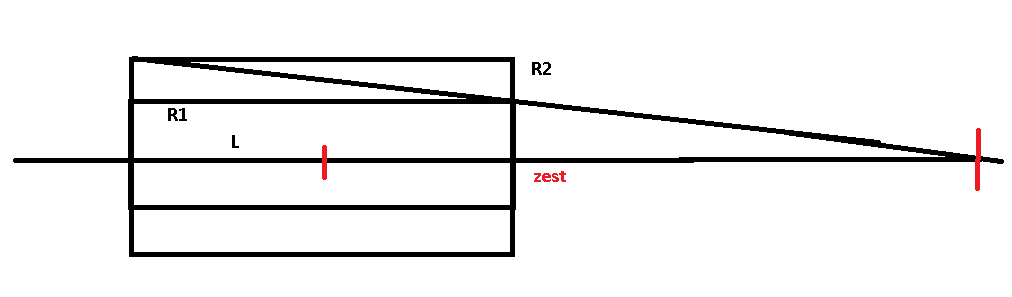
\includegraphics[scale=0.4]{vertice}
	\end{figure}
	\noindent
	Si vuole inoltre specificare che l'algoritmo è stato costruito in modo da selezionare il bin relativo al primo massimo dell'istogramma per determinare il valore di \textit{zrec} in caso sia presente più di un massimo. 
	
	\item \textit{plot()}: è impiegata per lo studio dell' efficienza e risoluzione dell'algoritmo di ricostruzione. Le vengono passati dei vector contenenti la coordinata \textit{z} dei punti ricostruiti e quella del vertice primario $z_{true}$, la molteplicità e l'errore in \textit{z} del vertice ricostruito. Con queste informazioni si riempono gli istogrammi relativi ai residui, all'efficienza rispetto alla molteplicità e a $z_{true}$ e alla risoluzione rispetto alla molteplicità e $z_{true}$. I risultati ottenuti sono salvati nel file \textit{istogrammi.root}. 
\end{itemize}

\subsection{Macro canvasses}
La macro \textit{canvasses.C} è utilizzata per eseguire i plot degli istogrammi contenuti in \textit{istogrammi.root} e applicare un fit gaussiano sui residui. 
\\
Questa macro contiene anche la funzione \textit{SetmyIsto()} per impostare stile, titoli e range degli istogrammi.

\newpage
\section{Risultati}
A titolo esemplificativo si riporta di seguito uno degli istogrammi utilizzati per valutare il valore di $z_{rec}$. Tale istogramma è riferito a una simulazione di 100000 eventi in cui è stata considerata come distribuzione di molteplicità quella assegnata.
\begin{figure}[H]
	\centering
	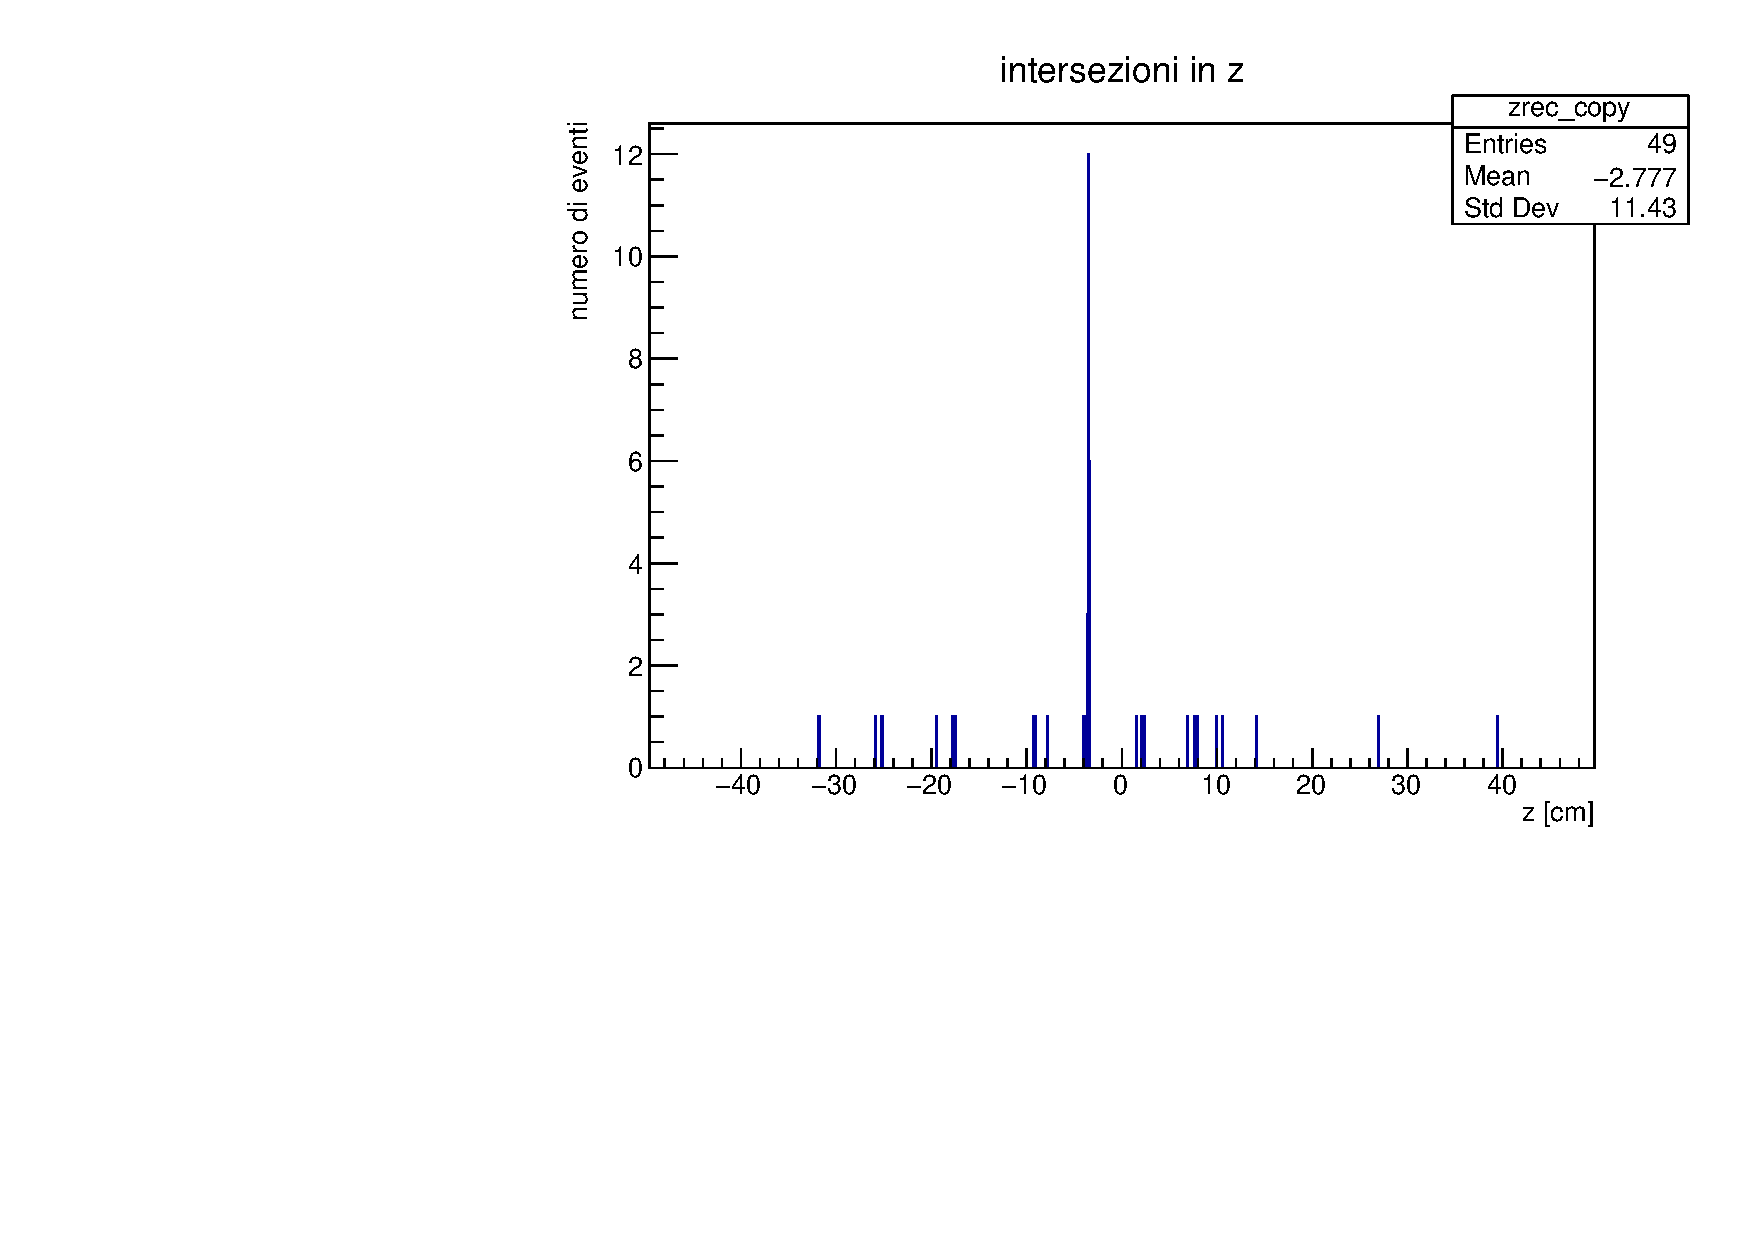
\includegraphics[scale=0.35]{istofuncintersezioni}
\end{figure}
\noindent
Per quanto riguarda i risultati ottenuti in funzione della molteplicità, risulta evidente che l'andamento dei residui totali non segua una distribuzione gaussiana, mentre i residui relativi a eventi con molteplicità simile (fra 3 e 5 o fra 45 e 55) lo fanno.

\begin{figure}[!htb]
	\minipage{0.32\textwidth}
	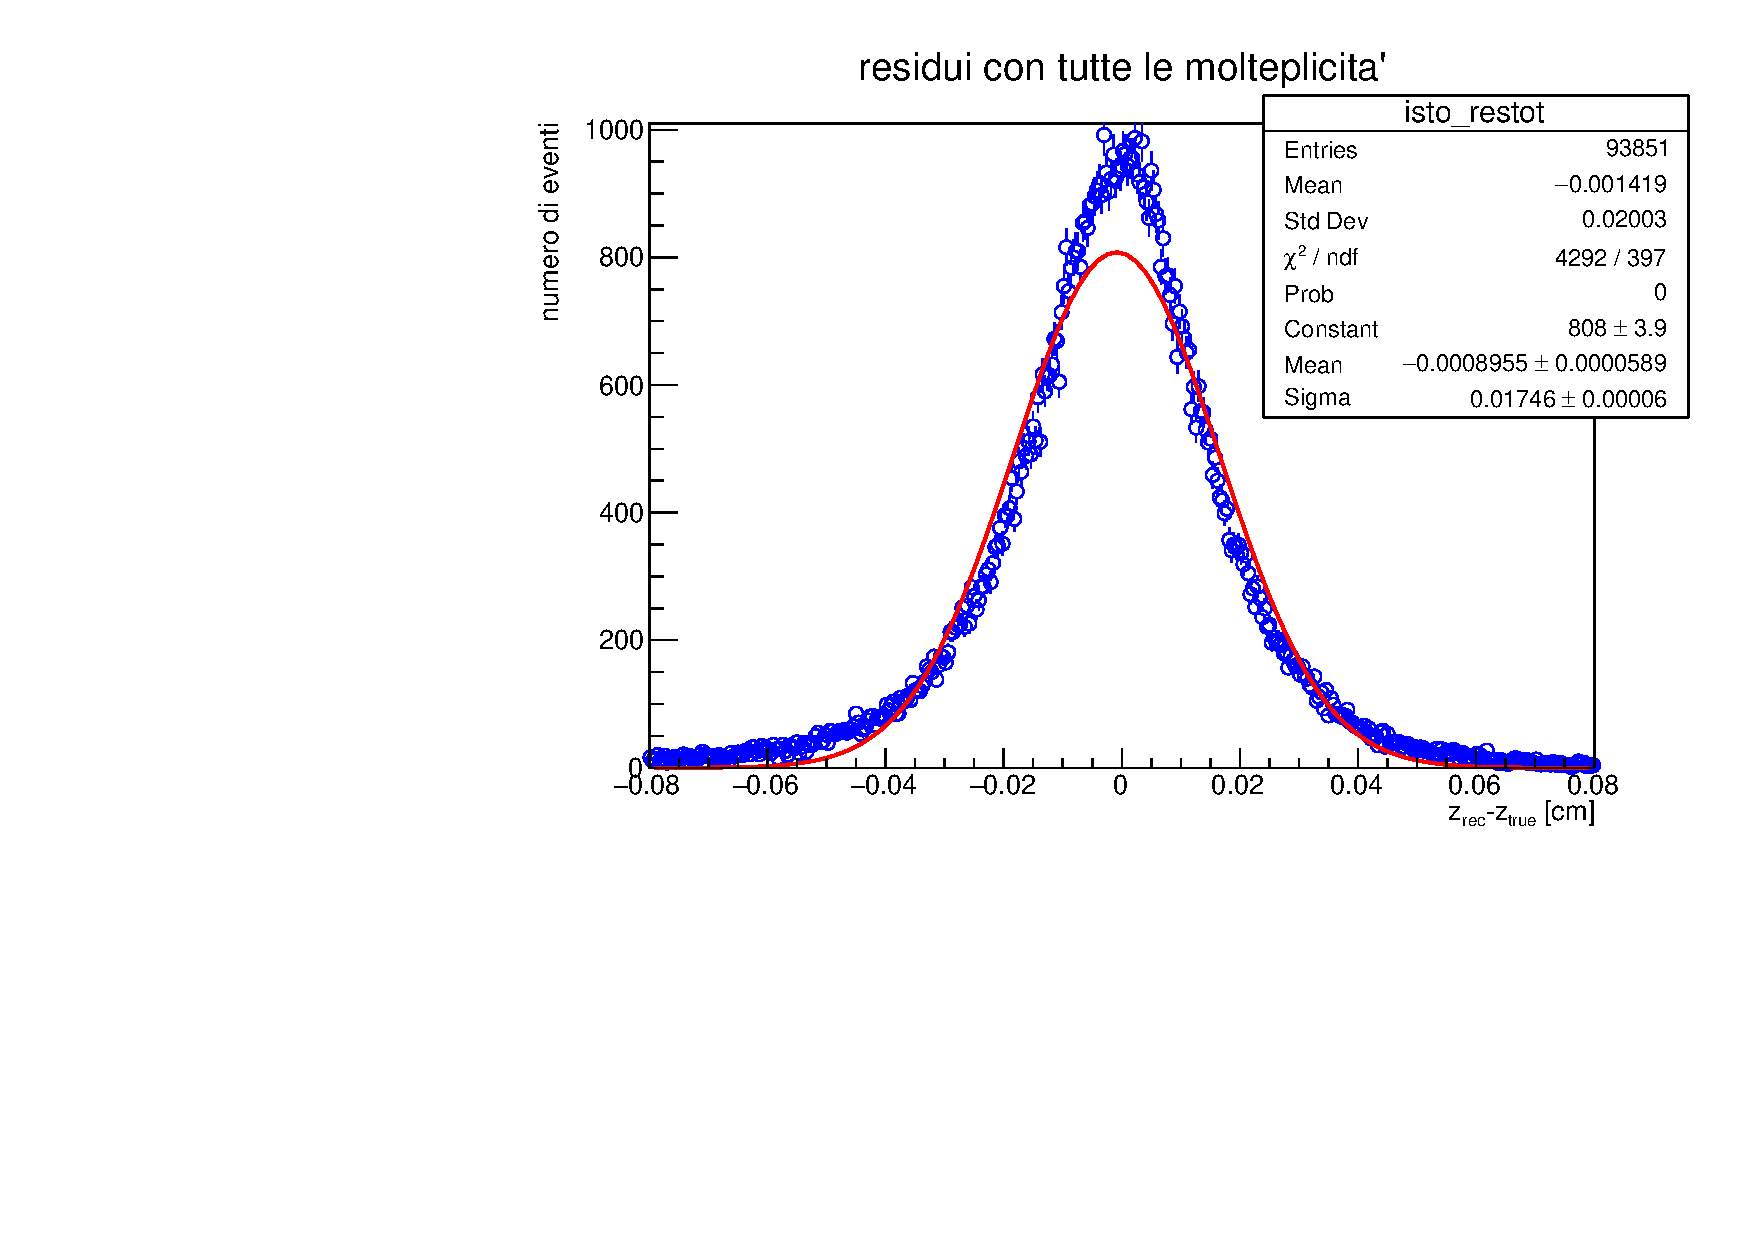
\includegraphics[scale=0.28]{restot}
	
	\endminipage\hfill
	\minipage{0.32\textwidth}
	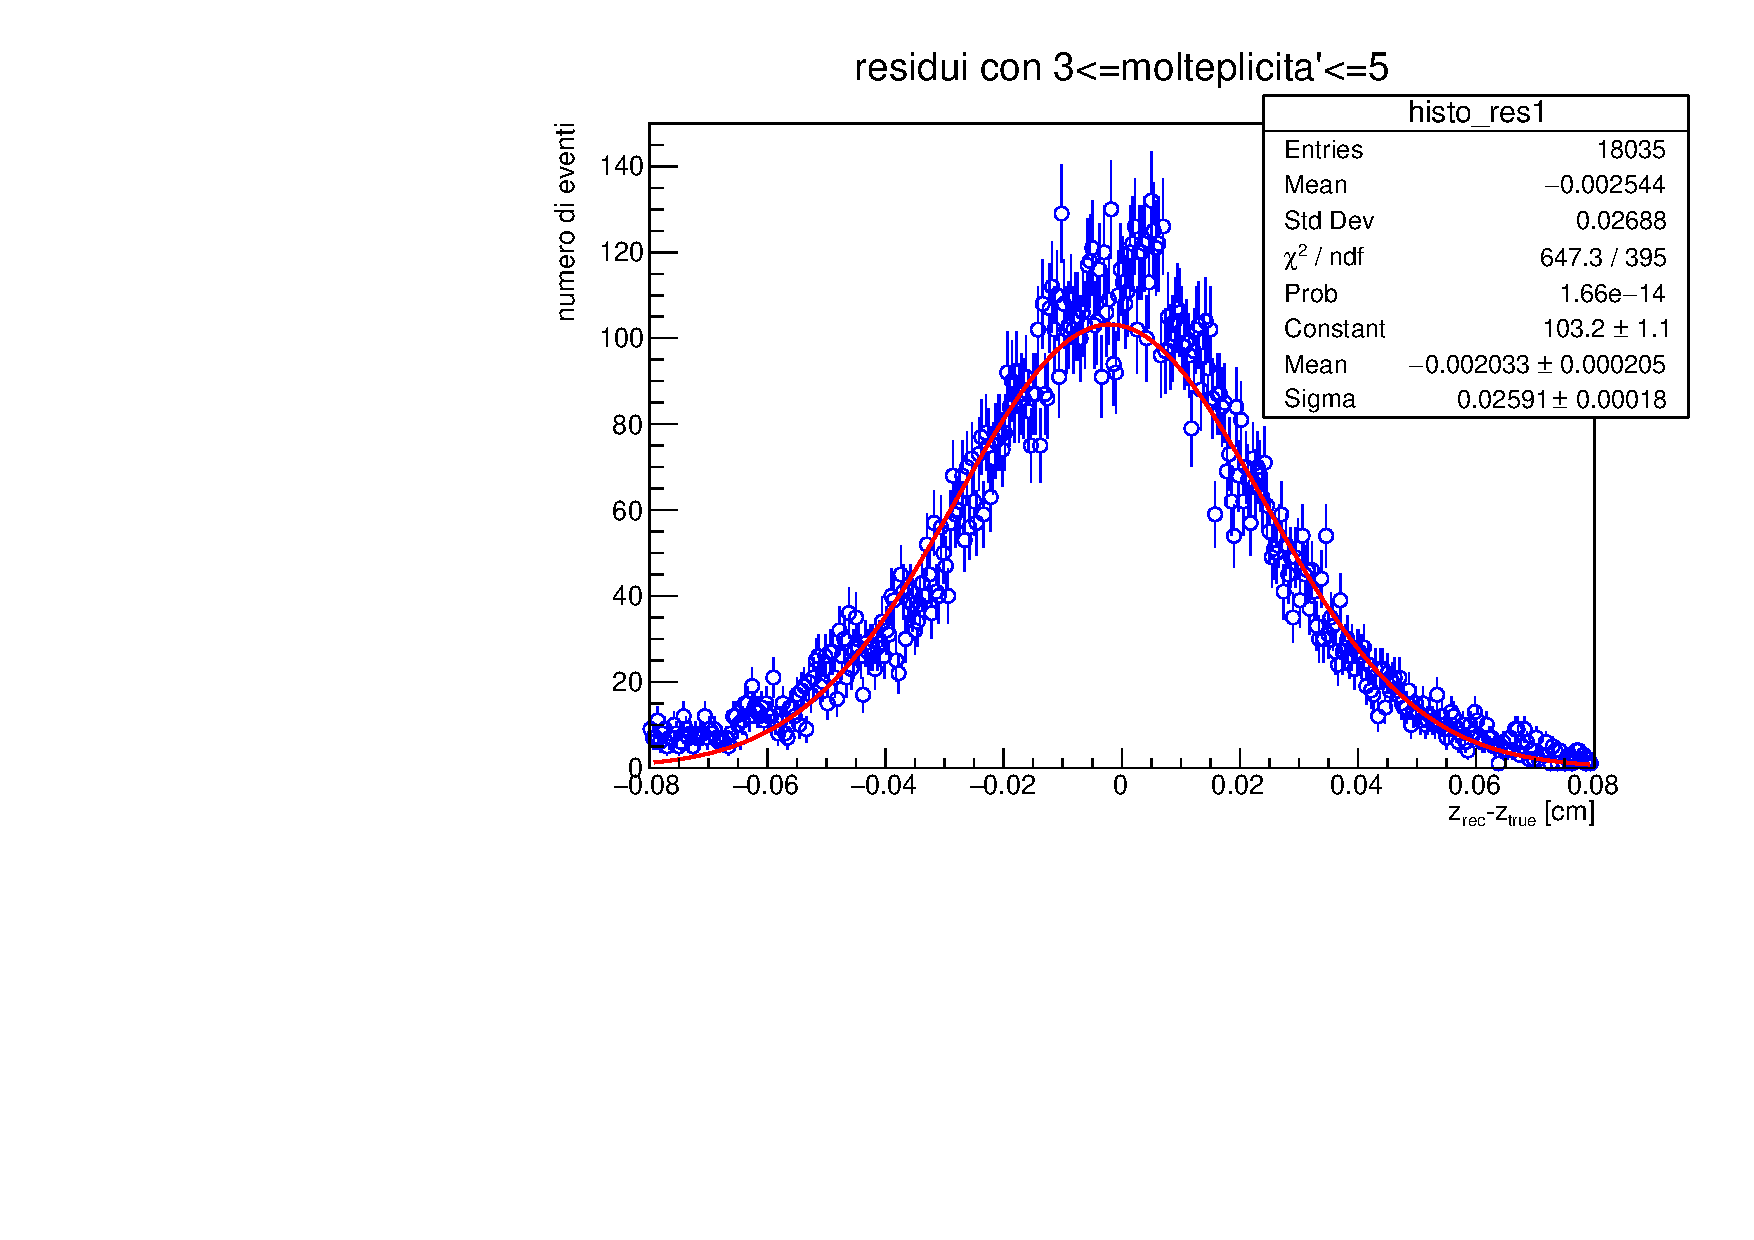
\includegraphics[scale=0.29]{resbassemult}
	
	\endminipage\hfill
	\minipage{0.32\textwidth}%
	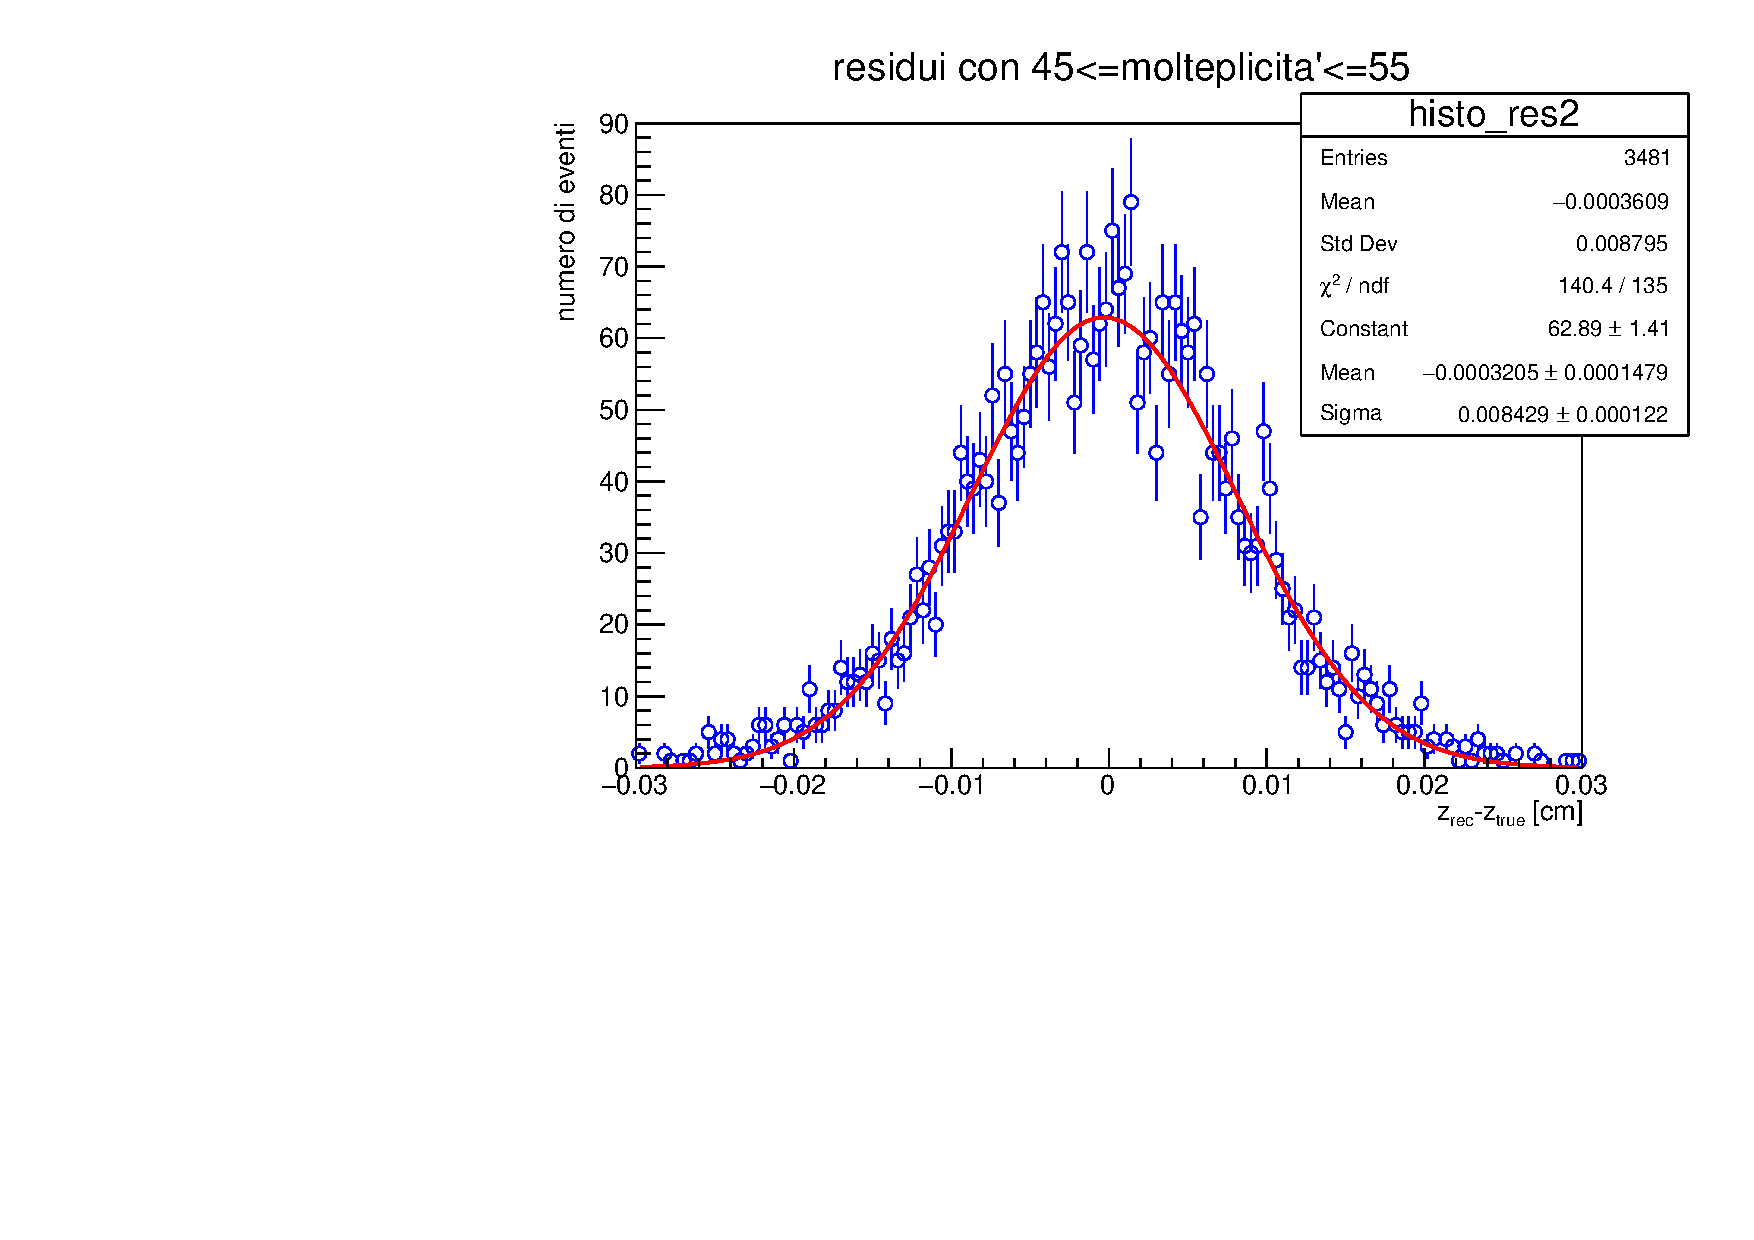
\includegraphics[scale=0.3]{resaltamult}
	
	\endminipage
\end{figure}
\noindent
Sono stati anche analizzati gli istogrammi dei residui bin per bin utilizzati per ricostruire la risoluzione in funzione della molteplicità, che è valutata come l'RMS di tali istogrammi. Sono tutti centrati in $0$ e con una larghezza di $100-400 \mu m$, come atteso da un valido algoritmo di ricostruzione.
\begin{figure}[H]
	\centering
	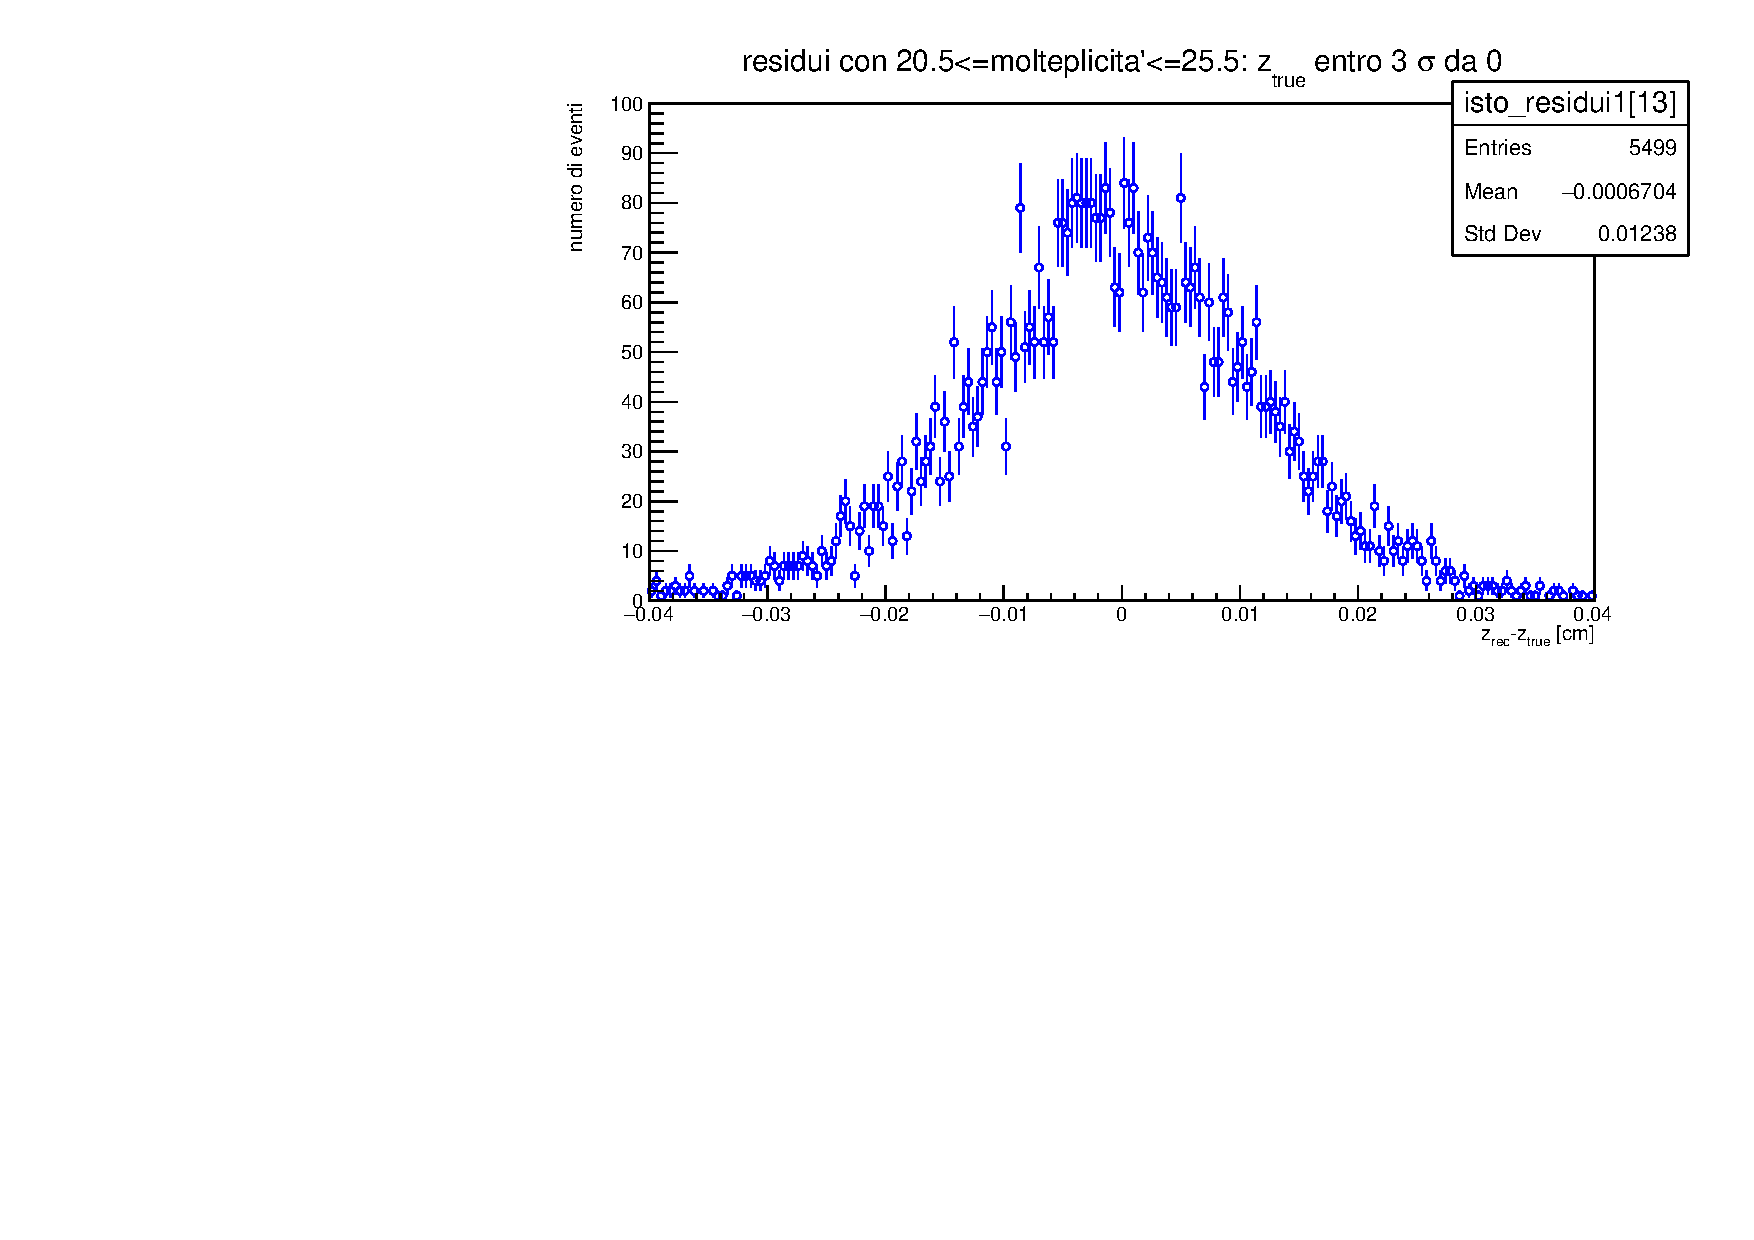
\includegraphics[scale=0.5]{resmulti20}

\end{figure}
\noindent
Per quato riguarda l'efficenza, considerando un valore di $z_{true}$ entro 3$\sigma$ da $0$ e entro 1$\sigma$ da 0 ($\sigma$=5.3 cm), si osserva che questa cresce con la molteplicità convergendo a 1 per molteplicità $>15$ circa.
Eè da notare che prima di tale convergenza la curva per 3$\sigma$ è leggermente più bassa di quella per 1$\sigma$, come atteso dal fatto che la prima contiene anche eventi molto lontani dal centro del rivelatore.
\begin{figure}[H]
	\minipage{0.5\textwidth}
	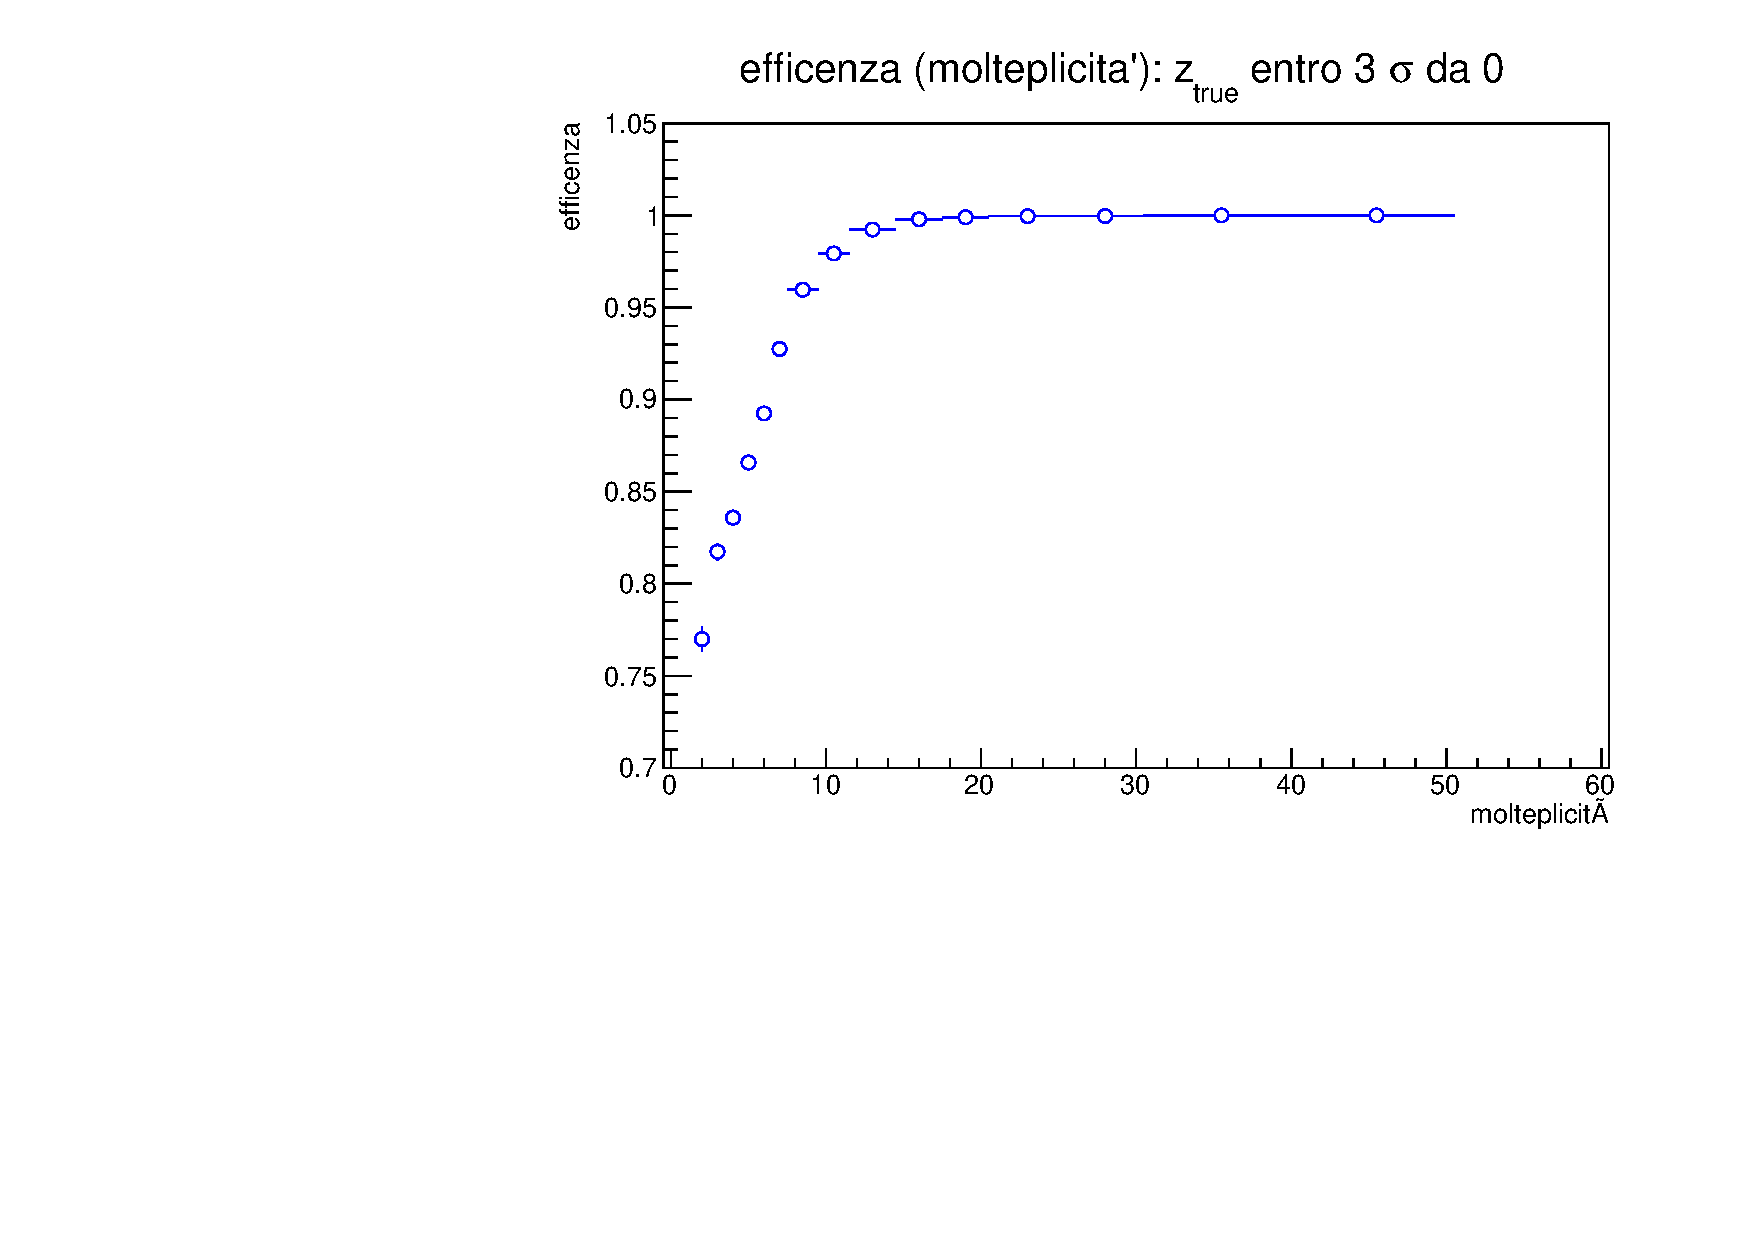
\includegraphics[scale=0.4]{effmultifunc3sigma}
	
	\endminipage\hfill
	\minipage{0.5\textwidth}
	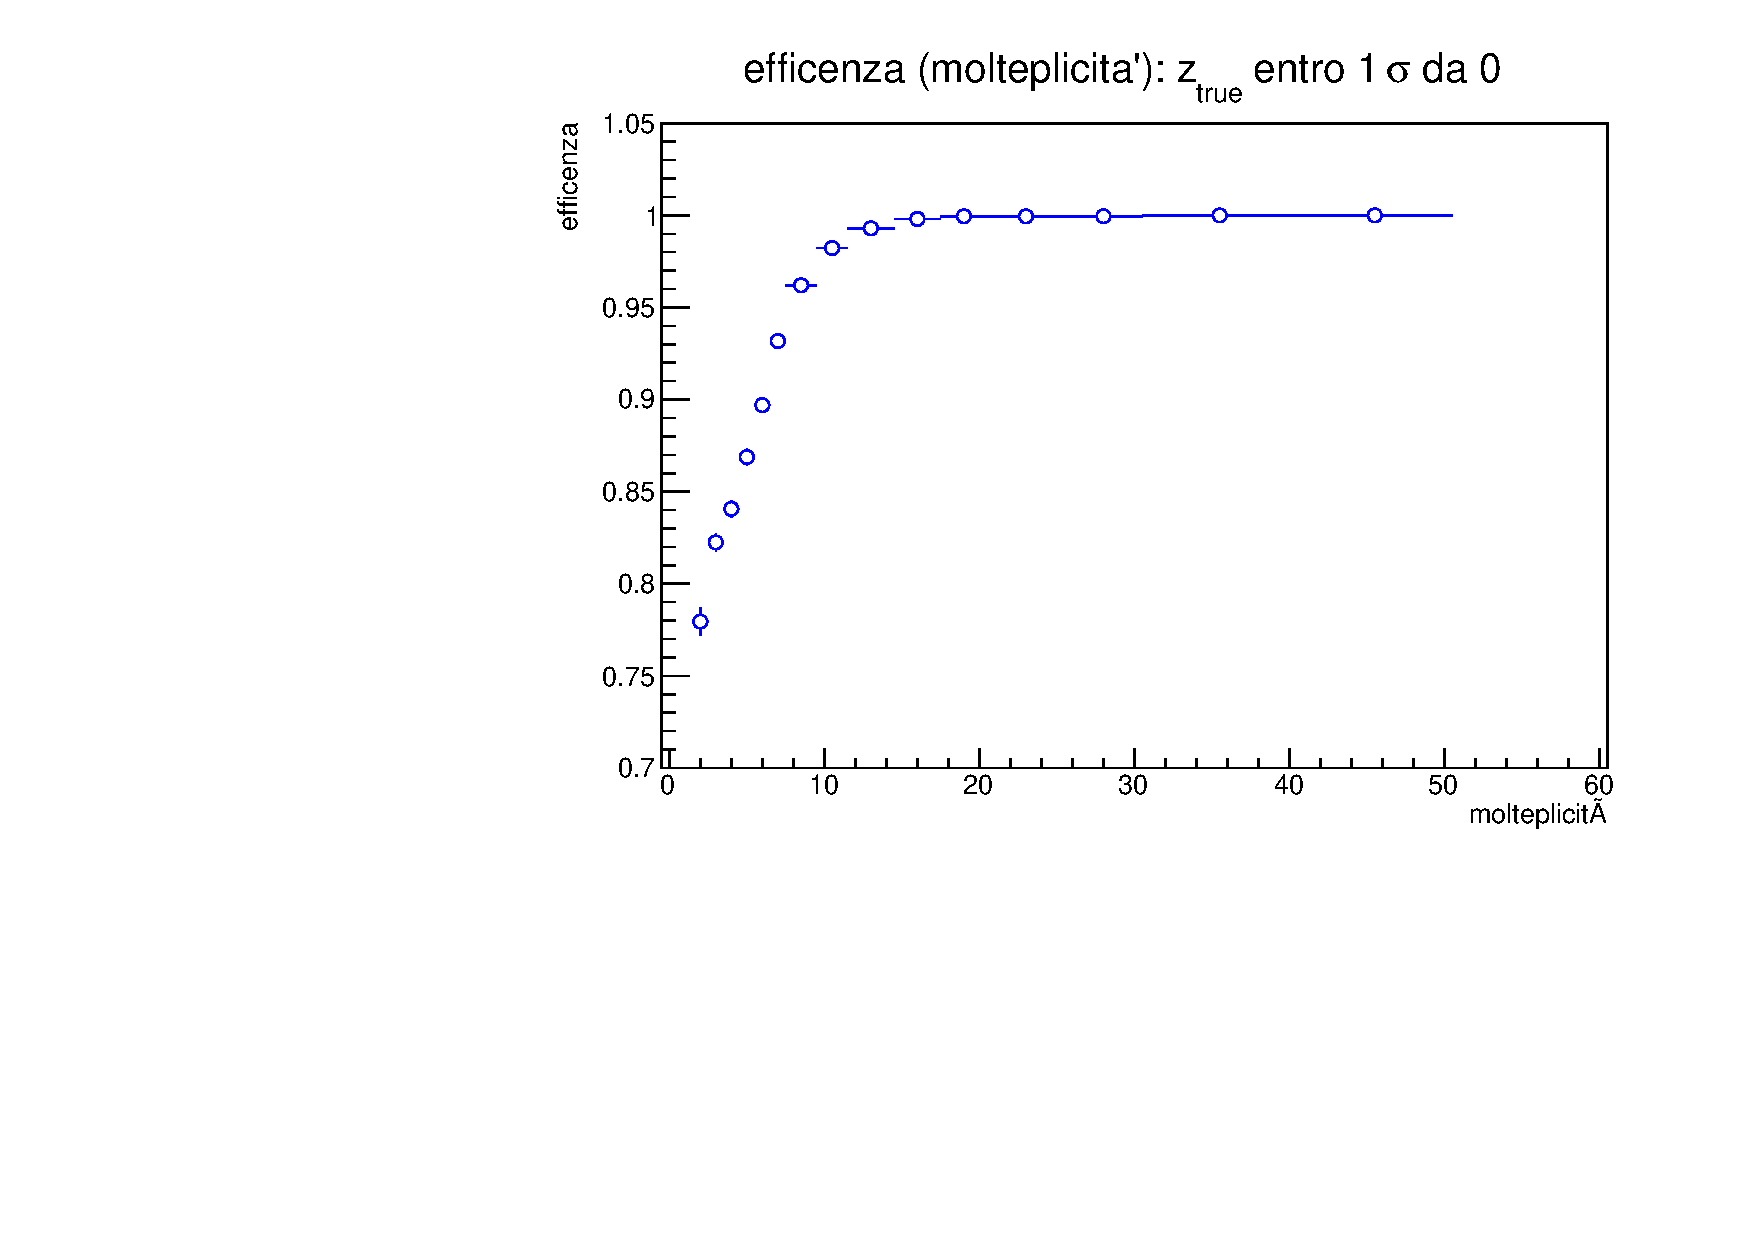
\includegraphics[scale=0.42]{effmultifunc1sigma}
	
	\endminipage
	
	
\end{figure}
\noindent
L'andamento della risoluzione è, come atteso, decrescente con la molteplicità (più tracce si hanno meglio si determina il vertice).Per il motivo già citato per l'efficenza, si osserva che la curva per 3$\sigma$ è un po' più alta (vertice determinato meno bene) rispetto a quella per 1$\sigma$.

\begin{figure}[H]
	\minipage{0.5\textwidth}
	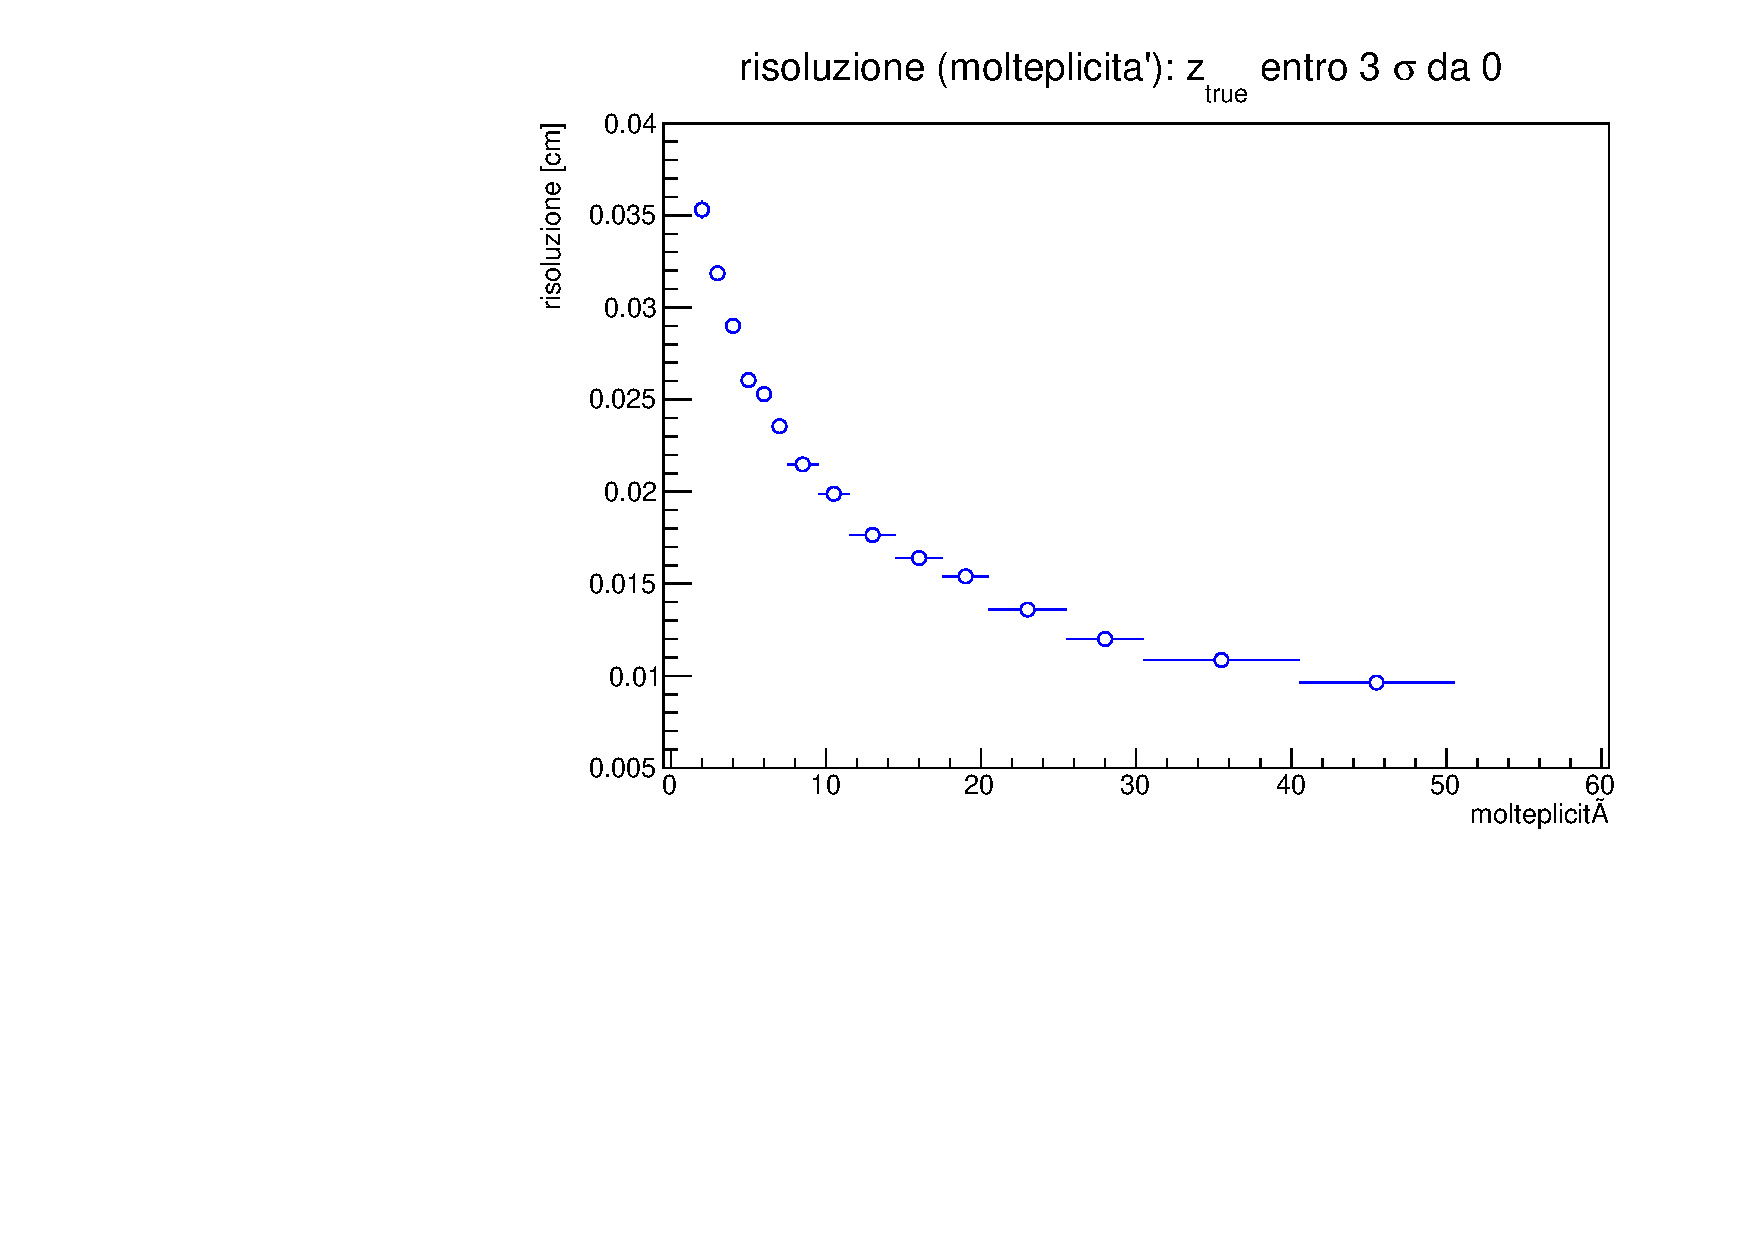
\includegraphics[scale=0.4]{rismultifunc3sigma}
	
	\endminipage\hfill
	\minipage{0.5\textwidth}
	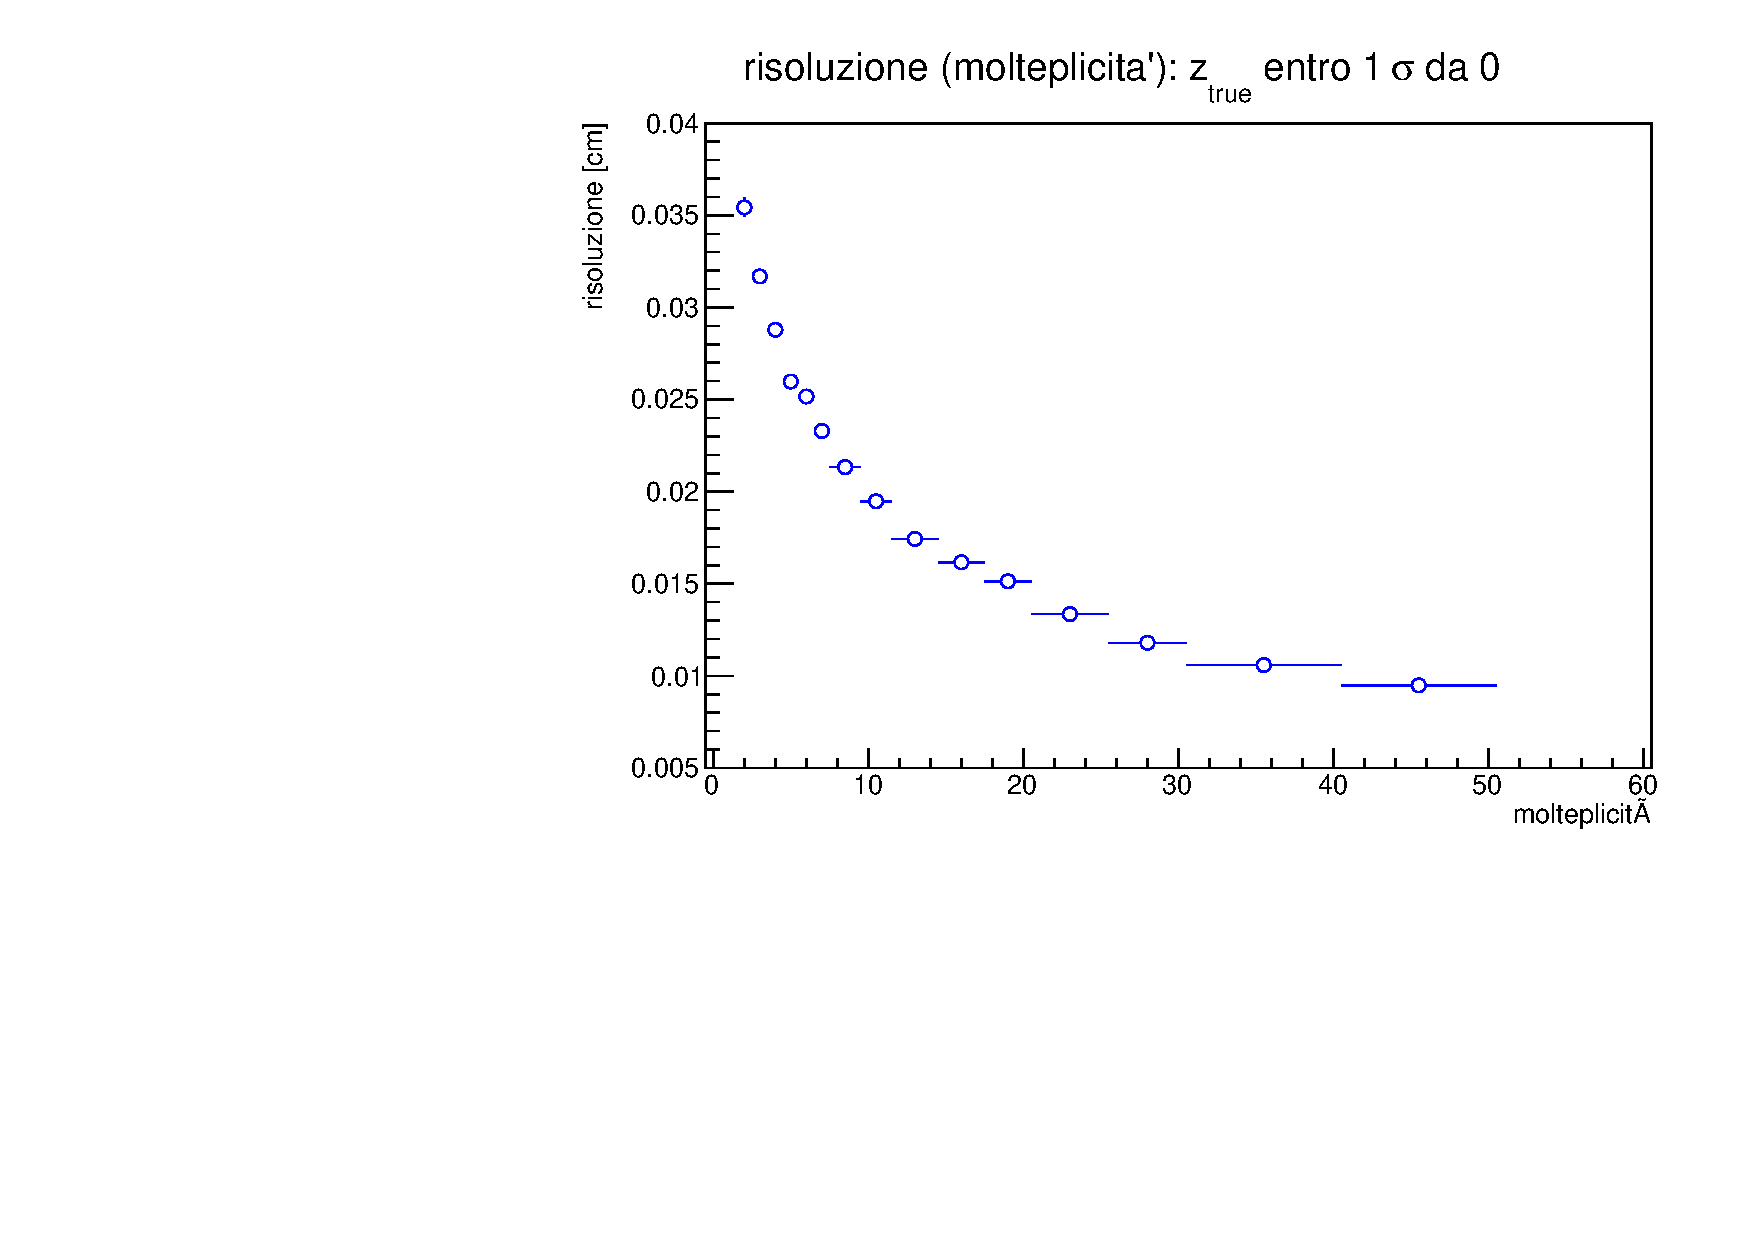
\includegraphics[scale=0.42]{rismultifunc1sigma}
	
	\endminipage
	
	
\end{figure}
\noindent
Le stesse analisi sono state nello studio dei risultati in funzione di $z_{true}$.
\\
Per quanto riguarda i residui, si ottengono andamenti analoghi a quelli ottenuti in funzione della molteplicità.
\begin{figure}[H]
	\centering
	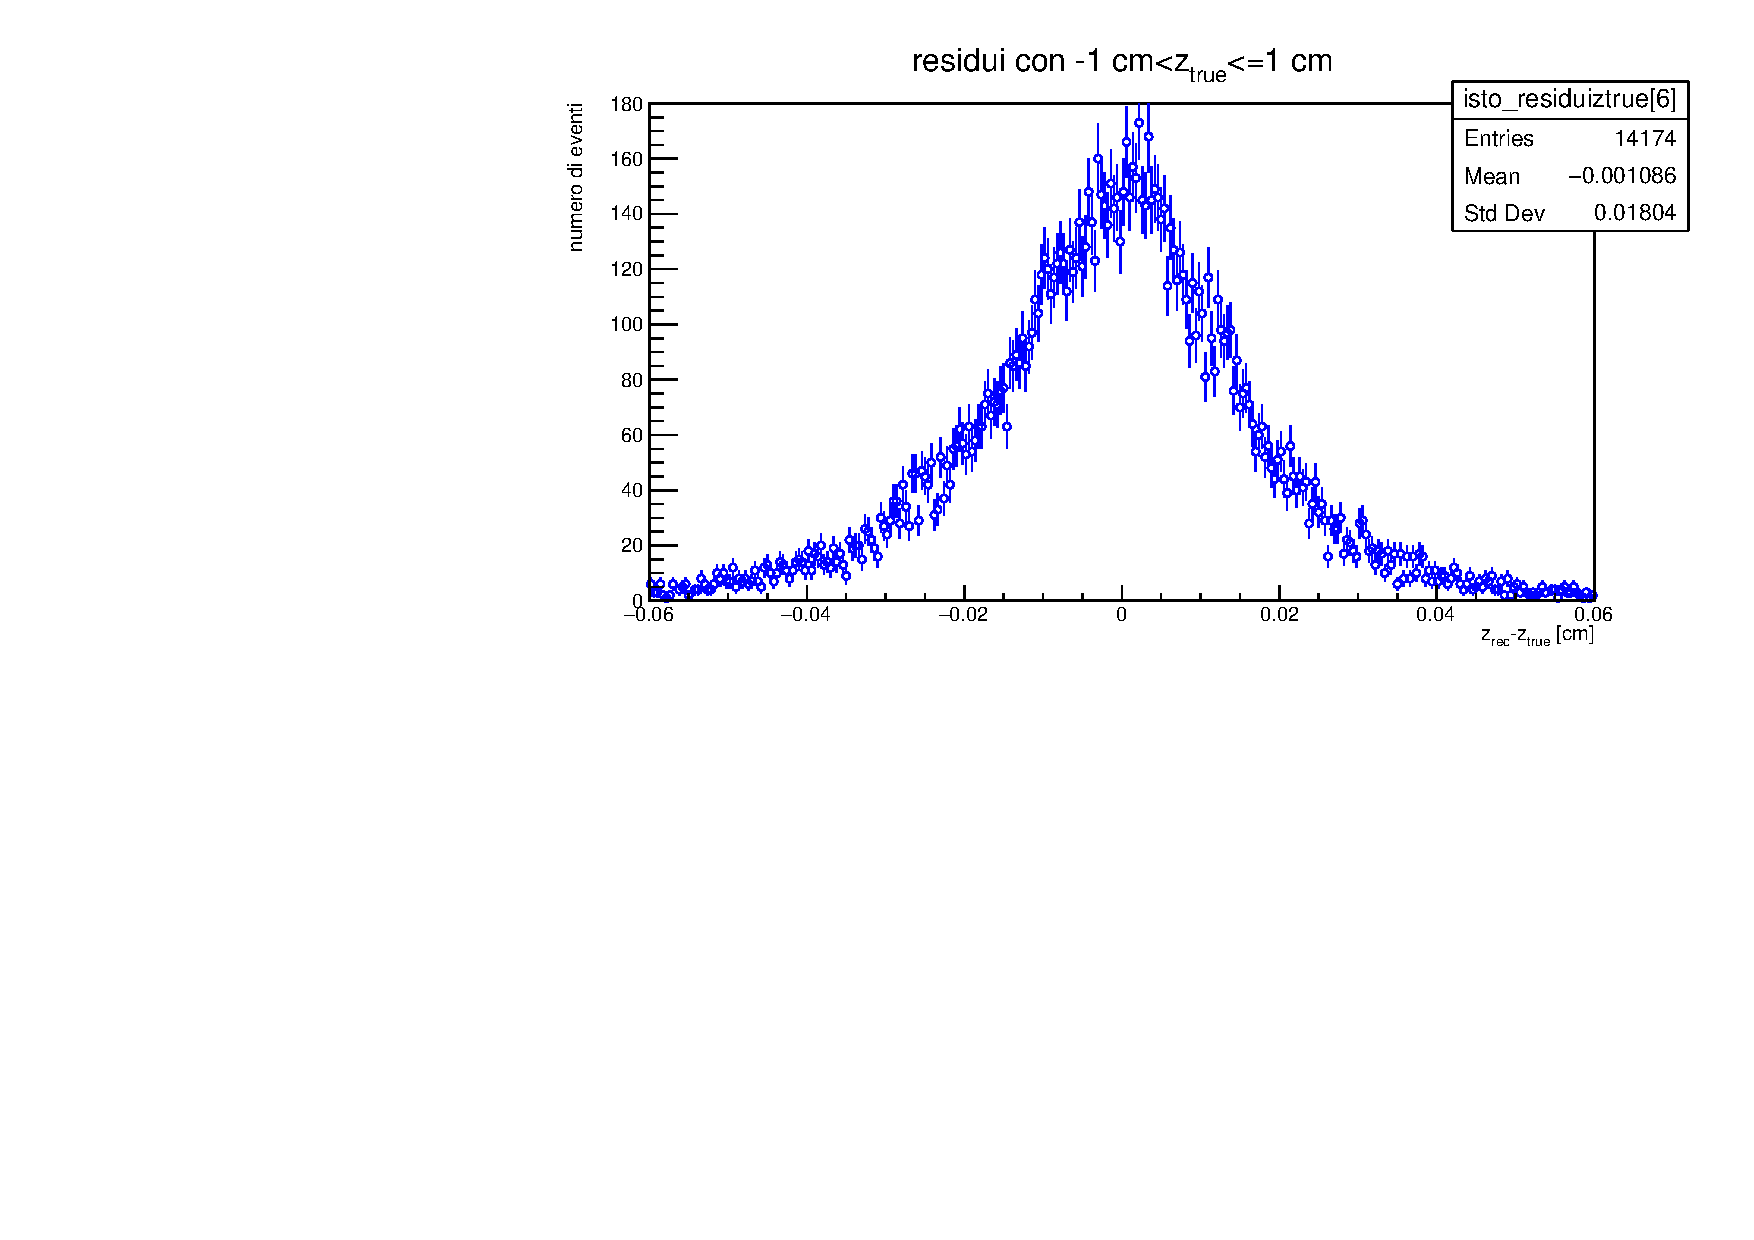
\includegraphics[scale=0.5]{resztrue}
\end{figure}
\noindent
L' andamento dell'efficienza riporta un massimo in $0$ e decresce ai lati (come atteso visto che molti degli eventi generati più esternamente producono tracce che escono dall'apparato). Per la risoluzione risulta l'andamento opposto: si ha il minimo in $0$ e l'andamento cresce ai lati.
\begin{figure}[H]
	\minipage{0.5\textwidth}
	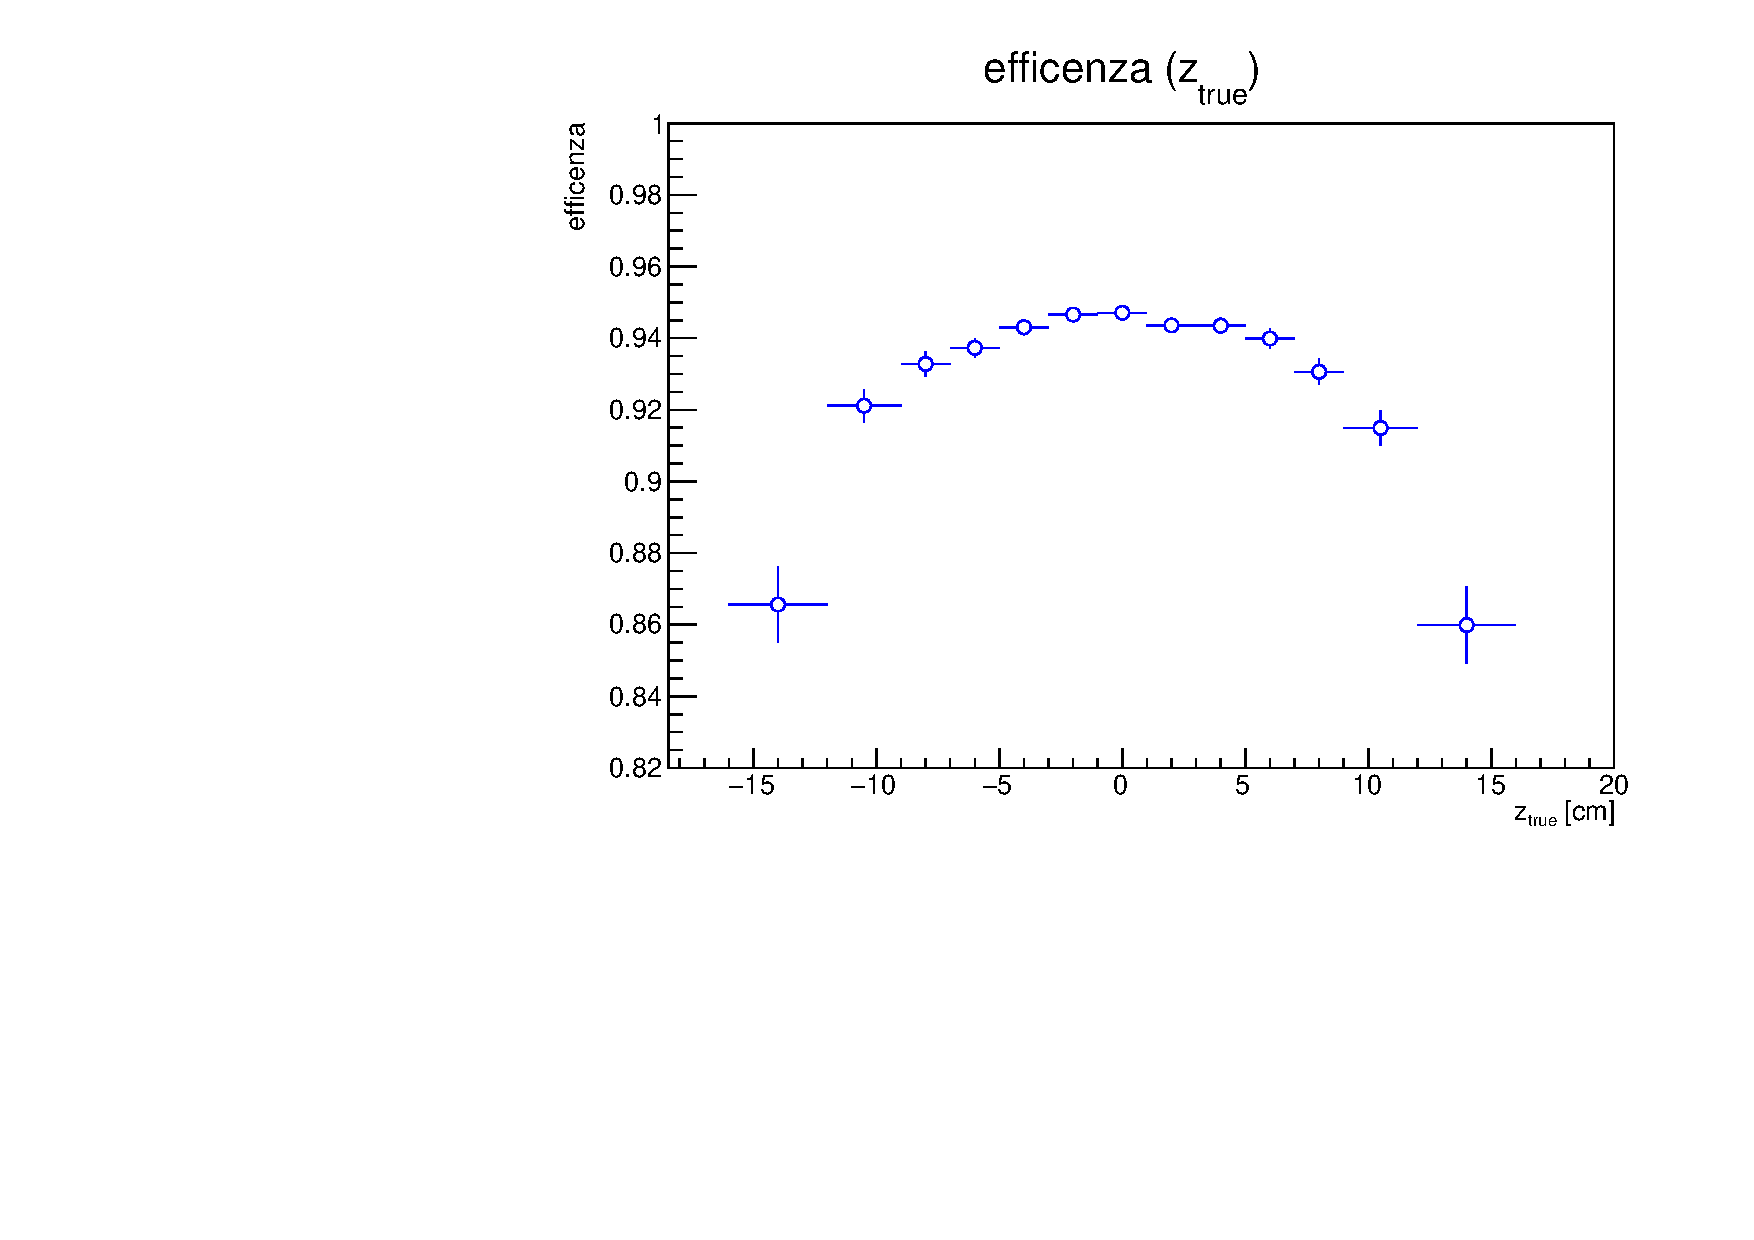
\includegraphics[scale=0.4]{effztruefunc}
	
	\endminipage\hfill
	\minipage{0.5\textwidth}
	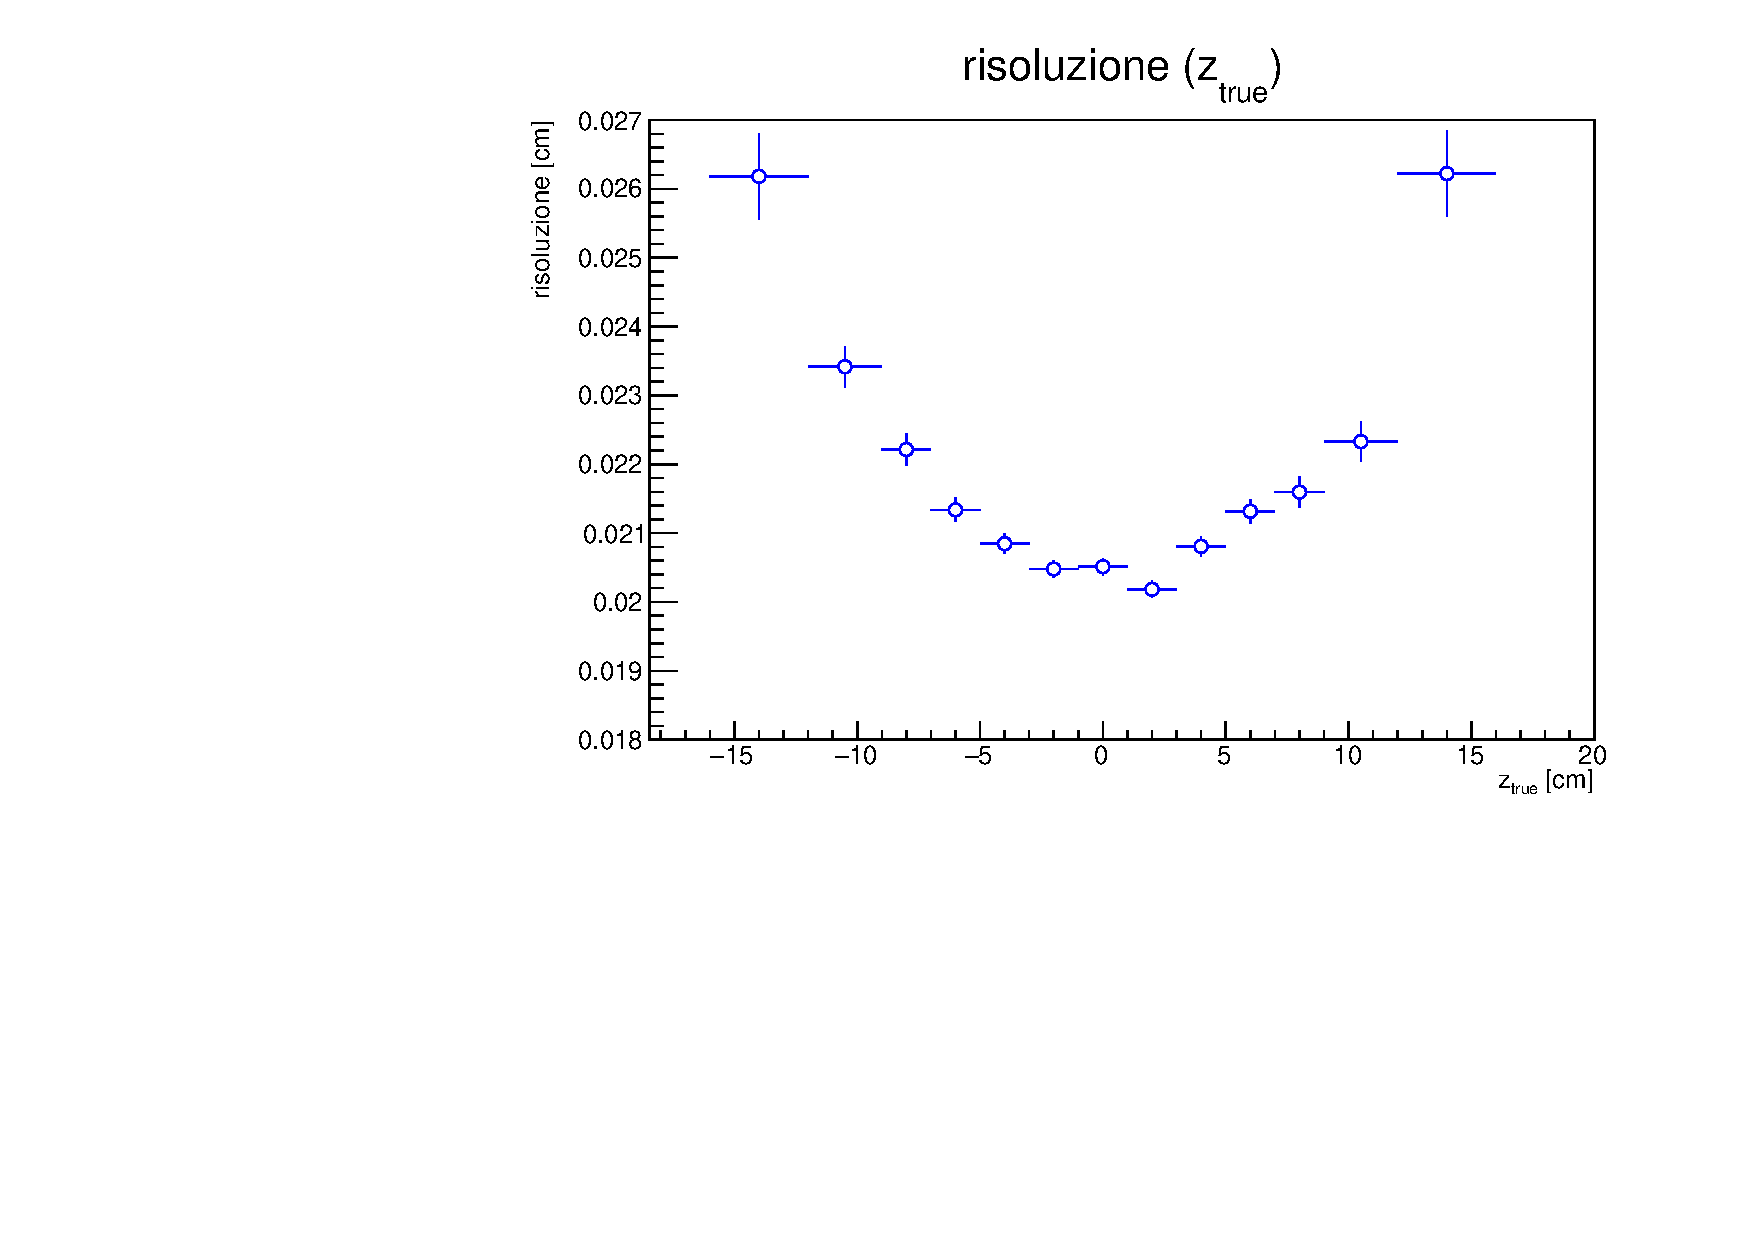
\includegraphics[scale=0.42]{risztruefunc}
	
	\endminipage


\end{figure}
\noindent
Le piccole deviazioni osservate rispetto ai risultati attesi si imputano a una bassa statistica (a seguito di rispetute simulazioni).


\end{document}
